\chapter{Objetivos}\label{cap.objetivos}
Una vez explicado el contexto de este proyecto, se describirán en este capítulo los objetivos, los requisitos y la metodología que se han empleado.\\

\section{Objetivos}

El propósito principal de este proyecto es la creación o mejora de tres prácticas para el entorno docente JdeRobot-Academy. En concreto mejorar una práctica de navegación global, crear una práctica de una aspiradora robótica y, por último, crear una práctica acerca del aparcamiento de coches autónomos. Siguiendo el diseño de JdeRobot-Academy, para cada práctica hay que desarrollar 4 ingredientes:

\begin{itemize}
\item Enunciado e infraestructura en el simulador
\item Componente académico que incluye \acrshort{gui} y código auxiliar
\item Solución de referencia
\item Evaluador automático
\end{itemize}

En cada una de estas prácticas se elaborará toda la infraestructura que se comunica con el Simulador Gazebo, donde el alumno podrá ver el resultado de la ejecución de su algoritmo. Se ofrecerá, en cada práctica, un fichero \textit{MyAlgorithm.py} donde el alumno programará su solución.\\

Lo que difiere en estas tres prácticas es el escenario de cada una de ellas, los diferentes elementos que se mostrarán en el interfaz gráfico, los elementos que tendrá en cuenta el evaluador automático a la hora de calcular la nota de cada alumno, y por último el algoritmo concreto de la solución. Cada una de ellas es un subobjetivo de este proyecto.\\

Primero, en la práctica ``TeleTaxi'' el objetivo es que el alumno aprenda técnicas de navegación global, en concreto, la técnica \textit{Gradient Path Planning}. Está práctica no es totalmente original, sino que existía una versión previa de la infraestructura y del componente académico, pero presentaban ciertos problemas. Por ello, en este proyecto se va a mejorar tanto la infraestructura como el componente académico, así como se va a desarrollar una nueva solución de referencia y un evaluador automático que nos permita calificarla.\\

Segundo, en la práctica ``Aspiradora Autónoma'' el principal objetivo es que el alumno sea capaz de proporcionar una solución para la limpieza de una casa sin autolocalización. En concreto, este algoritmo de referencia se basará en el que ejecutan los modelos de la serie 500 de Roomba de iRobot. Se realizará una solución que limpia en función de tres modos de navegación: giro en espiral, seguimiento de paredes y cruce de habitación. La aspiradora cuenta con diferentes sensores y actuadores, entre los que se encuentran un sensor láser, un sensor bumper, y actuadores que permiten dar órdenes a la aspiradora de velocidad de tracción y velocidad de giro.  En este caso la práctica se ha realizado desde cero, pues no existía una versión previa. Con ella los alumnos se familiarizarán con un problema robótico real, cotidiano y cuya solución ya se está comercializando.\\


En último lugar, en la práctica ``Aparcamiento Automático'' el propósito es la realización de una solución que sea capaz de aparcar un coche de forma autónoma. El coche está dotado de tres sensores láser (que se encuentran en la parte frontal, en la parte trasera y en el lateral derecho) para medir distancias a los coches y encontrar aparcamiento. La solución propuesta es una solución ``ad hoc'' basada en las medidas sensoriales que se obtienen de los láseres. La solución permite al vehículo encontrar una plaza de aparcamiento libre y realizar la maniobra de aparcamiento. Esta práctica, también realizada de cero, nos permitirá acercarnos a sistemas robóticos que ya existen en el mercado (Volkswagen Tiguan, etc) y con ello aprender cómo funcionan.

\section{Requisitos}
El desarrollo del proyecto estará guiado por los subobjetivos mencionados anteriormente y deberá ajustarse a los requisitos de partida del proyecto, los cuales hacen que la solución esté condicionada. Estos requisitos son:

\begin{enumerate}[1.]
\item Todas las simulaciones se realizarán en el simulador Gazebo, en concreto en la versión 7. Los modelos de robots que se emplearán serán creados. En este caso se utilizarán dos taxis (los cuales tienen diferentes sensores) y el modelo Roomba.
\item Se hará uso del \textit{middleware} robótico JdeRobot en su versión 5.5.2, que se explicará con detalle en el Capítulo~\ref{cap.infraestructura}. El uso de esta plataforma simplifica el desarrollo del comportamiento del robot. 
\item El sistema operativo que se empleará para este proyecto será Ubuntu 16.04.
\item El lenguaje de desarrollo empleado para crear los \textit{plugins} necesarios será C++. Sin embargo, en el resto de componentes se utilizará el lenguaje Python 2. Por compatibilidad con JdeRobot-5.5.2 y de éste con el \textit{middleware} ROS Kinetic no se ha usado Python-3.X, sino que se sigue Python-2.7.
\item Las soluciones han de ser vivaces. Los algoritmos propuestos no pueden detenerse mucho tiempo a pensar cuál será el próximo movimiento del robot, porque han de reaccionar rápido, en tiempo real y con movimientos suaves.
\end{enumerate}

\section{Metodología}
En el desarrollo del proyecto se ha seguido una metodología iterativa, donde cada iteración se compone de varias fases: determinar objetivos, planificación, diseño e implementación, análisis de riesgos, así como reuniones periódicas con el tutor.\\

Se ha optado por seguir el modelo de desarrollo en espiral, creado por Barry Boehm~\cite{modelo_espiral}~\cite{modelo_espiral1}. Este modelo se adapta perfectamente a este tipo de proyectos, ya que permite separar el comportamiento final en varias subtareas más sencillas para después juntarlas. Este modelo permite una gran flexibilidad ante cambios en los requisitos, algo bastante común.\\

Este modelo de ciclo de vida permite ir obteniendo prototipos funcionales, a la vez que se realiza el desarrollo del producto de forma incremental. El modelo consta de iteraciones, que se pueden llamar ciclos. En cada ciclo existen cuatro fases bien diferenciadas:

\begin{itemize}
\item Determinar objetivos: Se definen los objetivos específicos que deben cumplirse para que el ciclo actual pueda considerarse finalizado en base a los objetivos finales. Conforme vayan sucediéndose más iteraciones, los objetivos serán más complejos.
\item Análisis del riesgo: Se efectúa un análisis detallado para cada uno de los riesgos que pueda tener el objetivo fijado en la fase anterior. Se definen los pasos a seguir para minimizar los riesgos y después del análisis se planean estrategias alternativas.
\item Desarrollar y probar: Se desarrolla el producto o las partes del producto que se han acordado en las fases anteriores. Además, se llevarán a cabo las pruebas oportunas que permitan asegurar la calidad de la implementación, y que pueda seguir sirviendo en iteraciones futuras.
\item Planificación: Se revisan los resultados obtenidos mediante las pruebas de la fase anterior, y es donde se planifica la iteración siguiente teniendo en cuenta los posibles errores que se han cometido.
\end{itemize}

\begin{figure}[H]
  \begin{center}
    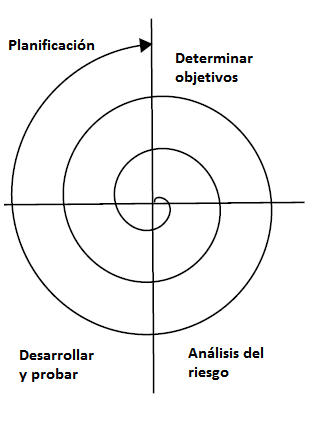
\includegraphics[width=0.4\textwidth]{figures/Objetivos/espiral.png}
		\caption{Modelo en espiral}
		\label{fig.espiral}
		\end{center}
\end{figure}

Para llevar a cabo esta metodología se han mantenido reuniones semanales con el tutor. En estas reuniones se analizaban los resultados de cada iteración, y en función de los resultados se fijaban nuevos objetivos y se planteaban posibles vías para resolverlos. El código que se ha ido desarrollando semanalmente se ha subido al repositorio propio público de Github \footnote{\url{https://github.com/RoboticsURJC-students/2016-tfg-vanessa-fernandez}}, que emplea el sistema de control de versiones. Además, las tareas realizadas se han ido mostrando semanalmente mediante explicaciones, vídeos o imágenes en la bitácora de la página de JdeRobot \footnote{\url{http://jderobot.org/Vmartinezf-tfg}}.\\

El resultado global de este TFG, las tres prácticas creadas, han sido integradas en el repositorio oficial de JdeRobot-Academy. Y están disponibles
como software libre.  

\section{Plan de trabajo}
Las etapas temporales en las que se ha dividido el proyecto, que además se corresponden con el modelo en espiral, son:

\begin{itemize}
\item Familiarización con el entorno JdeRobot y OpenCV. En esta etapa se ha descargado e instalado la plataforma JdeRobot, el entorno docente JdeRobot-Academy, y todo el software necesario para el desarrollo del proyecto. En esta fase se engloba el aprendizaje del uso de Github, para el control de versiones, y el aprendizaje básico de la librería OpenCV. Para cerrar esta fase se han realizado algunas soluciones de prácticas existentes del entorno JdeRobot-Academy.
\item Familiarización con el simulador Gazebo y sus \textit{plugins}. En esta etapa se ha estudiado código de la plataforma JdeRobot, así como el material disponible en Gazebo en la página oficial \footnote{\url{http://gazebosim.org/}}.  Además, se han realizado pruebas creando mundos simples en Gazebo mediante modelos ya disponibles. También se ha realizado un estudio de los \textit{plugins} creados en JdeRobot (compilación e instalación), aprendizaje básico de C++, y desarrollo de algún \textit{plugin} necesario para el desarrollo de las prácticas.
\item Desarrollo de la práctica ``TeleTaxi'': Desarrollo del enunciado, la infraestructura en gazebo, el componente académico, la solución de referencia y
el evaluador automático.
\item Desarrollo de la práctica ``Aspiradora Autónoma'': Desarrollo del enunciado, la infraestructura en gazebo, el componente académico, la solución de referencia y el evaluador automático.
\item Desarrollo de la práctica ``Aparcamiento automático'': Desarrollo del enunciado, la infraestructura en gazebo, el componente académico, la solución de referencia y el evaluador automático.
\end{itemize}